
\documentclass{article} % EXPAND THE PREAMBLE TO SEE ALL OF THE CODE
\usepackage[utf8]{inputenc}
\usepackage{amsmath, amsfonts} 
\allowdisplaybreaks
\usepackage{amssymb}
\usepackage{esint} % for more integral symbols
\usepackage[margin=1.75in]{geometry} % [margin=1.0in]
\usepackage{graphicx} % more arguments for the \includegraphics command
\usepackage{wrapfig} 
\usepackage{textcomp} % more text symbols
\usepackage{mwe} % used for idk?
\usepackage{gensymb} % for symbols (e.g \degree and \ohm)
\providecommand{\e}[1]{\ensuremath{\times 10^{#1}}}
\usepackage{multicol} % for columns
\usepackage{float} % to better format tables
\restylefloat{table} % to better format tables
\usepackage{tabularx} % to better format tables
\usepackage{titlesec} 
\usepackage{enumitem} % allows better formatting for list environments
\usepackage{tikz} % graphs and drawings
\newcommand{\comment}[1]{} % for multiline comments
\usepackage[stretch=10]{microtype} % best package ever
\usepackage{booktabs} % for all your fancy table needs
\usepackage{environ}
\usepackage{siunitx}
\usepackage{mathrsfs}
\usepackage{cancel}
\usepackage{multirow} % allows multirow cells in tables
\usepackage{xcolor} % fancier color options
\usepackage{tikz-qtree} % trees
\usepackage{forest} % more trees (better imo)
\usepackage{mathtools}
\usepackage{hyperref}

\usepackage{contour}
\usepackage{ulem}
\renewcommand{\ULdepth}{1.8pt}
\contourlength{0.8pt}

\newcommand{\myuline}[1]{
  \uline{\phantom{#1}}%
  \llap{\contour{white}{#1}}%
}



\renewcommand{\arraystretch}{1} 

\title{CS 451 Final Project}
\author{Zane Globus-O'Harra}
\date{\textit{23 March 2023}}

\begin{document}
\maketitle

\section{Cover Page}

\begin{itemize}
    \item \textbf{Author:} Zane Globus-O'Harra
    
    \item \textbf{Project Title:} Formula 1 Database

    \item \textbf{Connection Information}
    \begin{itemize}
        \item \textbf{Port Number:} 3372

        \item \textbf{Host Name:} ix

        \item \textbf{Guest Account Login \& Password:} 

        login: guest 

        password: guest 

        \item \textbf{Database Name:} f1db

    \end{itemize}

    \item \textbf{Project URL:} TODO

    \item \textbf{Highlights:} TODO
\end{itemize}

\section{Summary}

\subsection{High Level Overview}
The world that will be modeled will be a simplified version of a Formula
1 (F1) car-racing season. This will include the drivers, the teams the
drivers are in, the races, and the results of those races. 

\subsection{Kinds of Data}
The kinds of data that will be stored will be about the drivers, the
teams, and the results that those drivers receive in the races that they
participate in. I'm not sure how in-depth you want me to go when
discussing kinds of data, but I think that the high level overview and
the ER diagram in the Logical Design section make it fairly clear the
kinds of data that I will be keeping track of. 

\subsection{Application Programs}
The application programs that are desired are a way to summarize the
results in a season, and determine who was the champion for that season.
I also want to look at the average results of each driver, and give a
summary of their best and worst races in a season (if I add data for
multiple seasons, then I will also be able to look at their results
across their career).

Each team will have two drivers, and I will have a way to compare the
drivers of one team. I will also have a way to look at the results of a
team over a season (the team's results is the sum of the results of its
drivers), and the results of that team over its tenure in F1.


\section{Logical Design}

\begin{figure}[H]
    \centering
    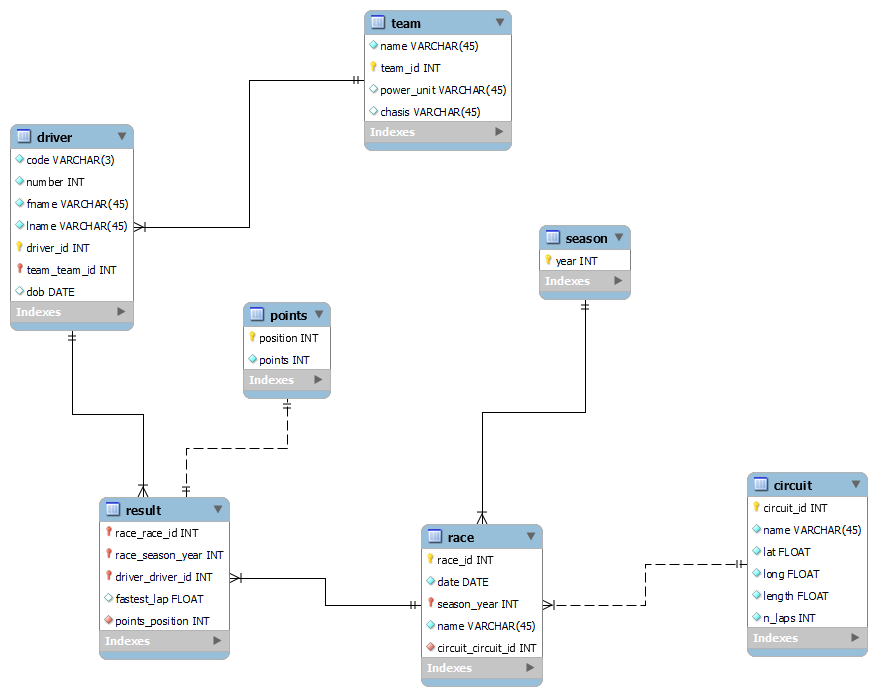
\includegraphics[scale=0.4]{f1db.png}
\end{figure}

\section{Physical Design}

Table names are in \textbf{bold and CAPITALIZED}, primary keys are
\myuline{underlined}, and foreign keys are \textit{italicized}. If an
attribute is a primary key and a foreign key, then it is
\myuline{\textit{underlined and italicized}}. Not
null requirements are indicated. Primary keys and foreign keys are
always not null.

\begin{itemize}
    \item \textbf{TEAM}: \myuline{team\_id}, name, power\_unit, chasis
    \begin{itemize}
        \item not null: power\_unit, chasis
    \end{itemize}

    \item \textbf{DRIVER}: \myuline{driver\_id},
    \textit{team\_team\_id}, code, number, fname, lname, dob
    \begin{itemize}
        \item not null: code, number, fname, lname
    \end{itemize}

    \item \textbf{RESULT}: \myuline{\textit{race\_race\_id}},
    \myuline{\textit{race\_season\_year}}, \myuline{\textit{driver\_driver\_id}},
    \textit{points\_position}, fastest\_lap

    \item \textbf{POINTS}: \myuline{position}, points
    \begin{itemize}
        \item not null: points
    \end{itemize}

    \item \textbf{RACE}: \myuline{race\_id},
    \myuline{\textit{season\_year}}, \textit{circuit\_circuit\_id},
    date, name 
    \begin{itemize}
        \item not null: date, name
    \end{itemize}

    \item \textbf{SEASON}: \myuline{year}

    \item \textbf{CIRCUIT}: \myuline{circuit\_id}, name, lat, long,
    length, n\_laps
    \begin{itemize}
        \item not null: name, lat, long, length, n\_laps
    \end{itemize}
\end{itemize}


\section{List of Applications}

\begin{enumerate}[label=(\arabic*)]
    \item 
    input: driver, season

    output: driver's race results across that season 

    \item
    input: season

    output: summary of the driver's results across that season

    \item
    input: season

    output: summary of the team (constructor) results of that season

    \item 
    input: driver, season

    output: best and worst results of that driver 

    \item 
    input: driver, season

    output: average results of that driver across that season

    \item 
    input: team, season

    output: average results of that team across that season

    \item 
    input: team, season 

    output: for each race in that season, compare the results of the
    drivers in that team

    \item 
    input: race, season 
    
    output: summary of the driver's results from that race in that season

    \item 
    input: race, season 
    
    output: summary of the team's results from that race in that season

\end{enumerate}


\section{User's Guide}

TODO

\section{Contents of Tables}

TODO

\section{Implementation Code}

TODO

\section{Conclusion}

TODO

\end{document}
